% !TEX root = ejemplo.tex

\chapter{Compilación y arara}
Como este documento puede ser compilado con Lua\LaTeX{} o pdf\LaTeX{} y tiene
paquetes diferentes para cada una de las anteriores, entonces el
pdf de salida depende de qué tipo de compilación se usó. Se recomienda que
si compila con un método y luego el otro sea haga una compilación
\enquote{nueva}, es decir, que antes de cambiar de
método se eliminen los archivos auxiliares para evitar posibles conflictos.

En este momento la compilación de nuestro ejemplo se ha vuelto algo complicada
y por tanto puede que tome algo de tiempo. Por ejemplo, para generar la tabla
de contenidos es necesaria la siguiente cadena
\begin{verbatim}
  lualatex ejemplo.tex
  lualatex ejemplo.tex
\end{verbatim}

En la sección~\ref{sec:bib} ya se había mencionado cuál es la cadena de
compilación para obtener la bibliografía. También vimos en el capítulo~\ref{cap:glos} que los glosarios requieren un paso más de compilación.

Si juntamos todos los pasos necesarios para obtener un pdf a partir de nuestros archivos, entonces obtenemos algo así:
\begin{verbatim}
  lualatex ejemplo.tex
  biber ejemplo
  makeglossaries ejemplo
  lualatex ejemplo.tex
  lualatex ejemplo.tex
\end{verbatim}
Como claramente tiene más pasos puede que haga el proceso algo lento.
Para hacer más rápida la compilación hay que evitar los pasos innecesarios.
Esto es, una vez que se ha compilado la primera vez se han creado los
archivos necesarios para componer bibliografía, glosarios, tabla de contenidos y
otros. Si no hay modificaciones a la bibliografía o glosarios, no es necesario
correr los pasos intermedios de arriba, ni tampoco correr tantas veces
\texttt{lualatex}. Para hacer esta compilación condicional escribimos
en las primeras líneas del archivo principal algo como lo siguiente
\begin{flushleft}
  \verb|% arara: ...|
\end{flushleft}
se usan para compilar con \texttt{arara} ya que se pueden agregar
condicionales de manera sencilla. Al menos mucho más simple que crear un
\texttt{latexmk} o un \texttt{makefile}. Aunque seguramente su instalación
local sí debe incluir \texttt{arara}, desgraciadamente overleaf no incluye
esta opción e ignorará los \textit{magic comments} del principio del archivo.
(Overleaf usa un \texttt{latexmk} para compilar, este método se asegura de
correr los pasos necesarios en cada compilación que hacemos.)

En el archivo \texttt{ejemplo.tex} se pueden ver los \textit{magic comments} al inicio del documento, estos son
\begin{verbatim}
% !TEX root = ejemplo.tex

% arara: lualatex: { draft: yes } unless changed(toFile('ejemplo.aux'))
% arara: biber if changed (toFile('refs.bib')) || found('log', 'Citation')
% arara: --> || found ('log', 'Please \\(re\\)run Biber')
% arara: makeglossaries if missing('gls')
% arara: --> || changed('glo') || changed(toFile('gloss.tex'))
% arara: lualatex: { synctex: yes } until !found('log', '\\(?(R|r)e\\)?run (to get|LaTeX)')
\end{verbatim}
El primero le dice a mi editor de texto cual es el archivo principal. Después
están las instrucciones de \texttt{arara}.

La primera instrucción con \texttt{arara} hace que compile con
\texttt{lualatex} el archivo \texttt{ejemplo.tex} con el modo \texttt{draft}.
Con esto sólo se crean los archivos auxiliares necesarios para generar el
documento. Al no crear un documento completo en esta compilación se gana un
poco de tiempo de compilación. Además sólo se hará está compilación si no
existe el archivo \texttt{ejemplo.aux}, ya que de existir es muy probable que
ya haya habido una compilación previa y existan los archivos necesarios para
una ompilación completa.

La segunda instrucción es una compilación condicional de \texttt{biber}. En
este caso sólo correrá \texttt{biber} si cambia el archivo \texttt{refs.bib} o
si en el \texttt{log} aparece la palabra \texttt{Citation} o cuando en este
mismo archivo se encuentran las palabras \texttt{rerun Biber}. Hay que notar
que \texttt{arara: -->} se usa como una continuación del comando anterior. En
nuestro caso \texttt{biber} usa dos líneas, lo mismo que
\texttt{makeglossaries}.

La tercera instrucción es la compilación condicional de
\texttt{makeglossaries}. Ahora sólo correra \texttt{makeglossaries} cuando no
exista un archivo \texttt{gls}, haya cambiado el archivo \texttt{glo} o haya
cambiado el archivo con nuestras entradas de los glosarios, \texttt{gloss.tex}.

Finalmente, compila el archivo \texttt{ejemplo.tex} con la opción \texttt{synctex}, para que se comuniquen el editor y el lector de pdf, y correrá \texttt{lualatex} tantas veces como sea necesario, es decir, cuando en el \texttt{log} ya no diga que hace falta correr de nuevo \texttt{lualatex} para generar alguna cita bibliográfica, entrada del índice o alguna referencia.

Ahora nuestro archivo se compila con el comando
\begin{verbatim}
  arara ejemplo
\end{verbatim}
Para mostrar cómo mejoró el tiempo de compilación la segunda
vez ponemos capturas de pantalla de la compilación de este documento, ver figuras.
Además muchos editores de \LaTeX{} pueden configurarse para compilar con
\texttt{arara}.  Por ejemplo, en Atom (el editor que uso) con el paquete atom-
latex se configura como \textit{custom toolchain} y el toolchain es:
\begin{verbatim}
  arara %DOC -v
\end{verbatim}

\begin{figure}[h]
\centering
  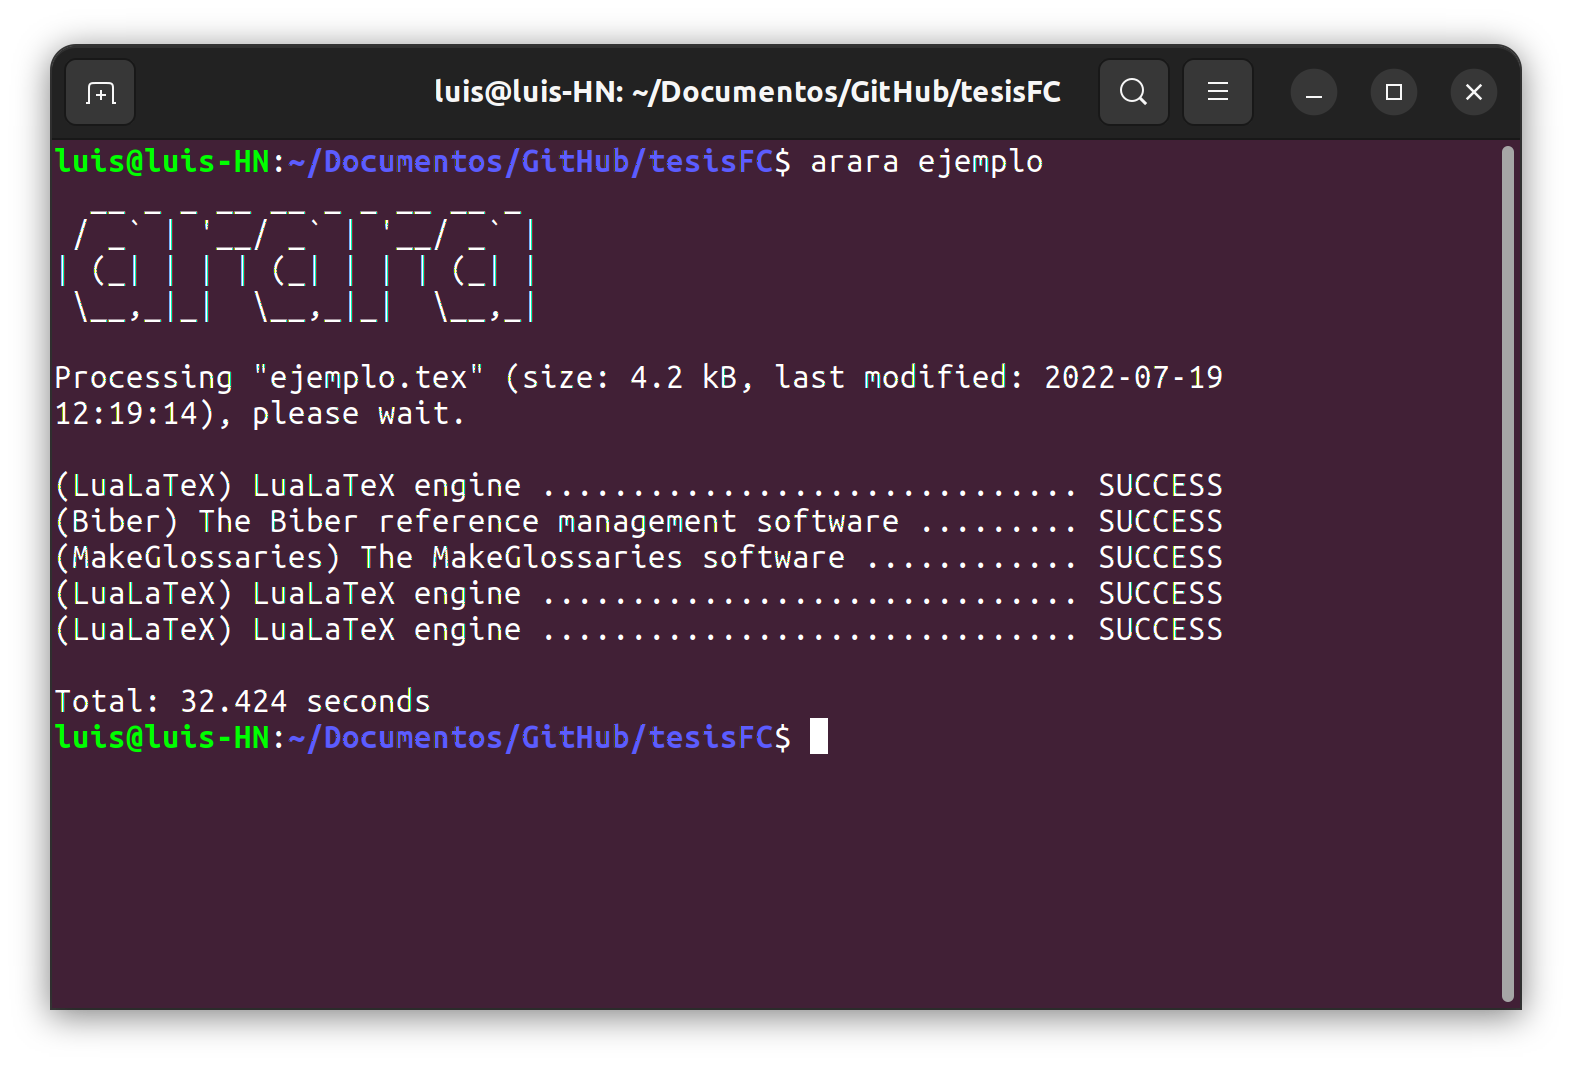
\includegraphics[width=0.7\linewidth]{primera}
  \caption{Primera compilación}
  \label{fig:primera}
\end{figure}

\begin{figure}[h]
\centering
  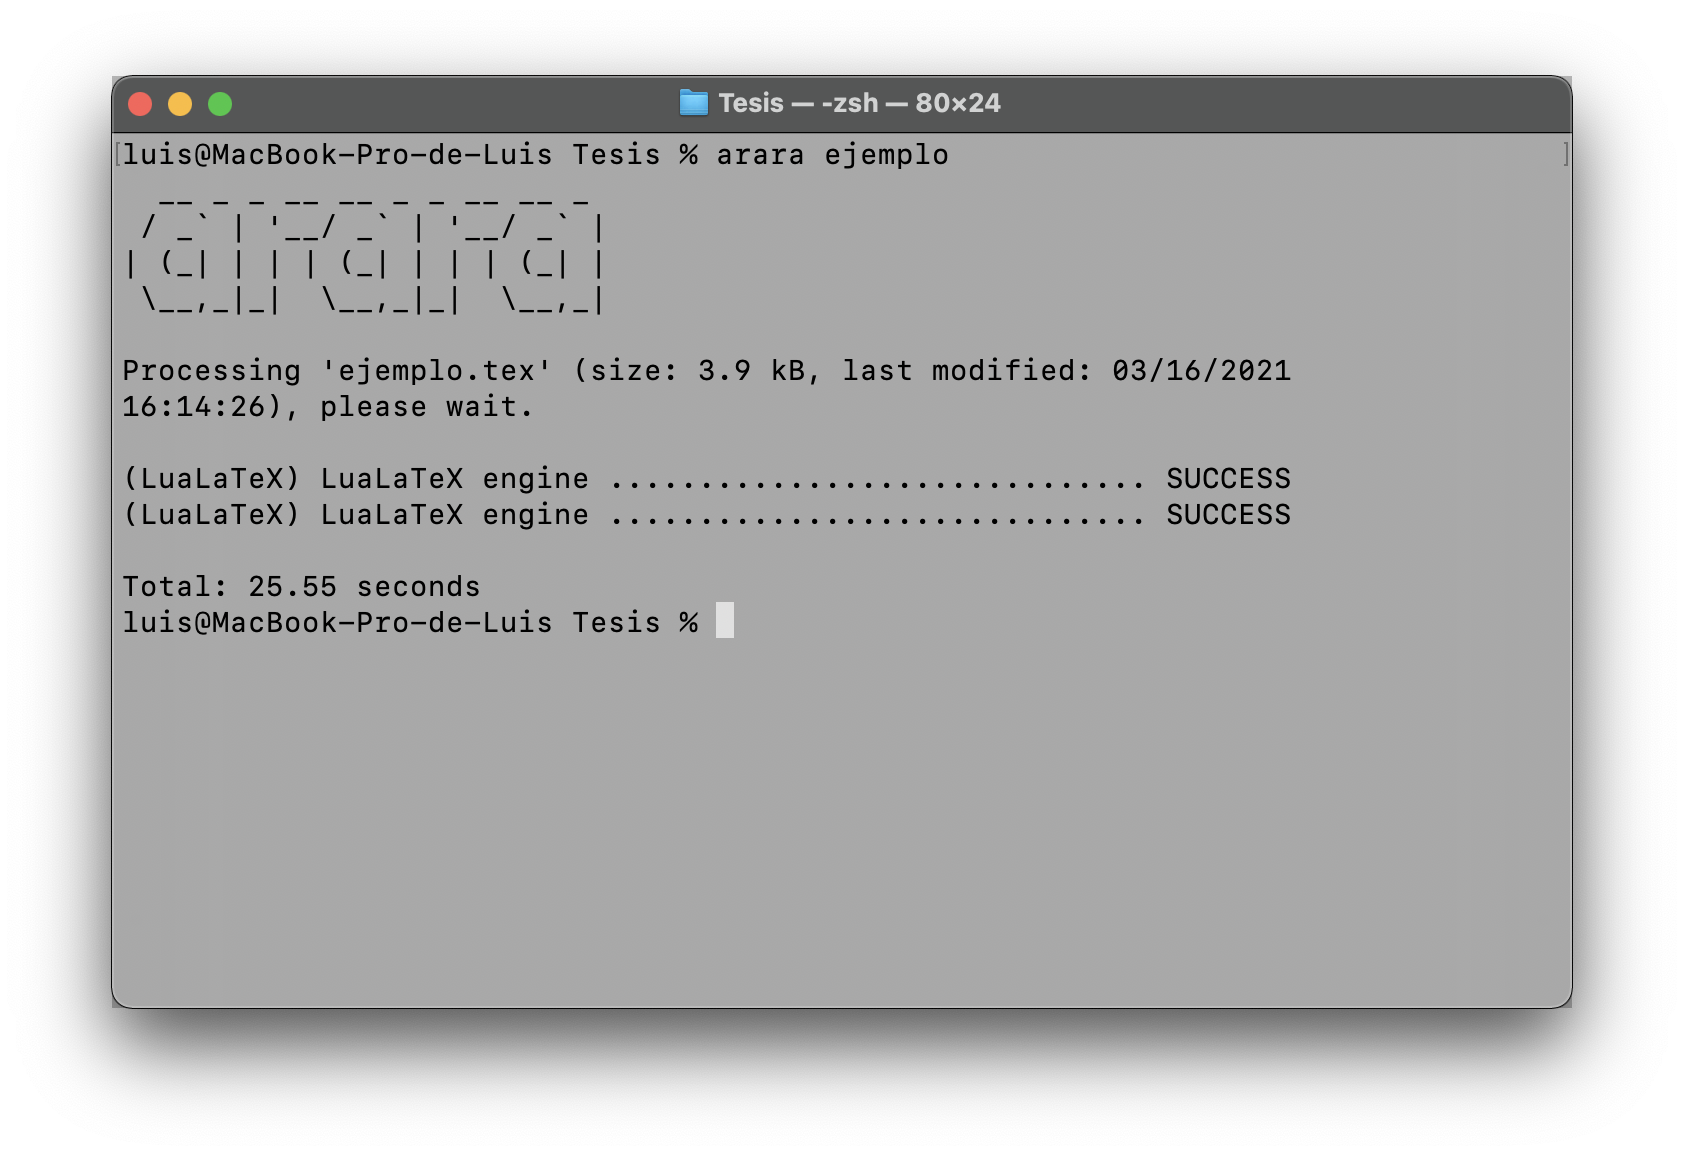
\includegraphics[width=0.7\linewidth]{segunda}
  \caption{Segunda compilación}
  \label{fig:segunda}
\end{figure}

Para configurarlo en TeXMaker hay que seguir las instrucciones en
\url{https://tex.stackexchange.com/a/107995}.

En TeXWorks: \url{https://tex.stackexchange.com/a/98795}.

En TeXShop: \url{https://tex.stackexchange.com/a/175673}.

Un último comentario acerca del tiempo de compilación es que en el proceso
de revisión y correcciones de la tesis, por ejemplo al revisar un capítulo
específico donde no se requiera estar viendo los otros, se puede escribir en
el preámbulo \verb|\includeonly{CapituloEnRevision}|. Una vez que ya haya
sido compilado el documento completo el comando anterior hará que sólo se
compile el capítulo en revisión con la paginación y las referencias a otros
capítulos correctas. Esto podría mejorar mucho el tiempo de compilación.
